\usetikzlibrary{calc}
\begin{frame}{ad injection (1)}
    \begin{itemize}
        \item internet advertising is big business
        \item \ldots{} but you need to pay websites to add ads?
        \item how about \myemph{modifying browser} to add/change ads
        \vspace{.5cm}
        \item mostly \myemph{bundled} with legitimate software
    \end{itemize}
\end{frame}


{ % all template changes are local to this group.
    \setbeamertemplate{navigation symbols}{}
    \begin{frame}[plain]
        \begin{tikzpicture}[remember picture,overlay]
            \node[at=(current page.center)] {
                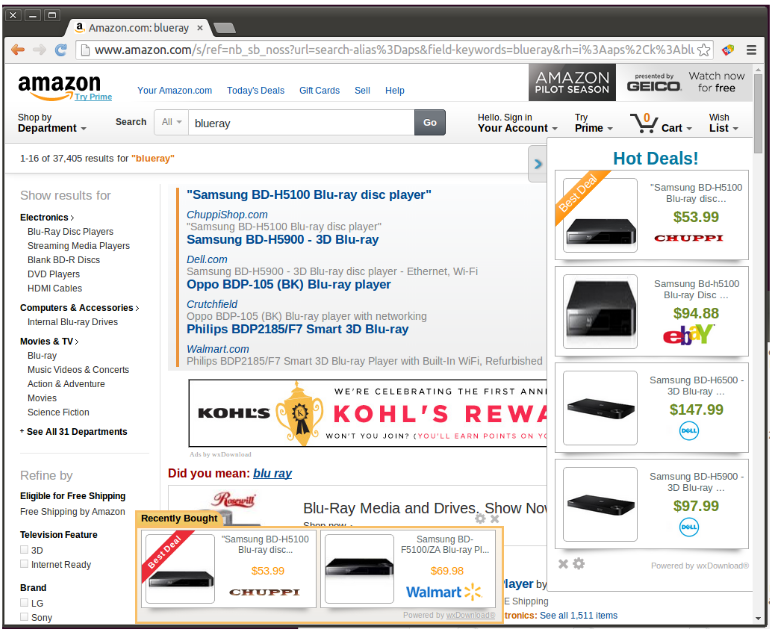
\includegraphics[height=0.96\paperheight]{../intro/ad-inject-amazon}
            };
        \end{tikzpicture}
    \imagecredit{From Thomas et al, ``Ad Injection at Scale: Assessing Deceptive Advertisement Modifications''}
    \end{frame}
}

\begin{frame}{ad injection (2)}
    \begin{itemize}
        \item 5\% of Google-accessing clients (2014)
        \item >90\% using code from VC-backed firm SuperFish:
        \vspace{.5cm}
            \item \$19.3 M in investment (CrunchBase)
            \item \$38M in revenue (Forbes, 2015)
            \item defunct after Lenovo root CA incident (2015)
            \item \ldots{} but founders reported started new, similar venture (JustVisual; according to TechCrunch)
    \end{itemize}
    \imagecredit{Adware prevalence: Thomas et al, ``Ad Injection at Scale: Assessing Deceptive Advertisement Modifications''}
\end{frame}

